

\chapter{Diseño e implementación} % Main chapter title

\label{Chapter3} % Change X to a consecutive number; for referencing this chapter elsewhere, use \ref{ChapterX}



En este capítulo se presentan los detalles del diseño de los nodos sensores y actuadores que conforman el trabajo, como así también los del software seleccionado.

\section{Arquitectura de la solución}
\label{sec:Arquitectura de la solución}

%Como se observa en la figura \ref{fig:blockdiagram}, el invernadero inteligente está compuesto por un conjunto de subsistemas encargados de las diferentes funciones de medición y control de variables, una aplicación central y un sistema que permita el acceso remoto de forma segura.

Para la implementación del prototipo propuesto en el trabajo se requirió la construcción de diferentes subsistemas encargados de las múltiples funciones dentro del invernadero inteligente. Cada uno de ellos opera en forma independiente del resto y se comunican con una aplicación central mediante una red inalámbrica. 
Para garantizar el acceso de los usuarios desde Internet se desarrolló una interfaz de acceso remoto.





\subsection{Componentes del sistema}
\label{Componentes del sistema}

En la figura \ref{fig:blockdiagram} se observa un diagrama en bloques de la arquitectura diseñada y sus componentes.

\begin{itemize}
\item El sistema de monitoreo y control de clima, organizado en dos bloques:
\begin{itemize}
\item Sensores de temperatura y humedad con sus correspondientes microcontroladores.
\item Unidad de control de temperatura formada por un microcontrolador, relé y ventiladores. 
\end{itemize}
Los sensores miden la temperatura y humedad ambiente en el invernadero y envían estas variables a la aplicación central por medio del microcontrolador. En base a los valores recibidos, la aplicación determina si es necesario emitir una señal para que la unidad de control de temperatura encienda los ventiladores.


\begin{figure}[h]
	\centering
	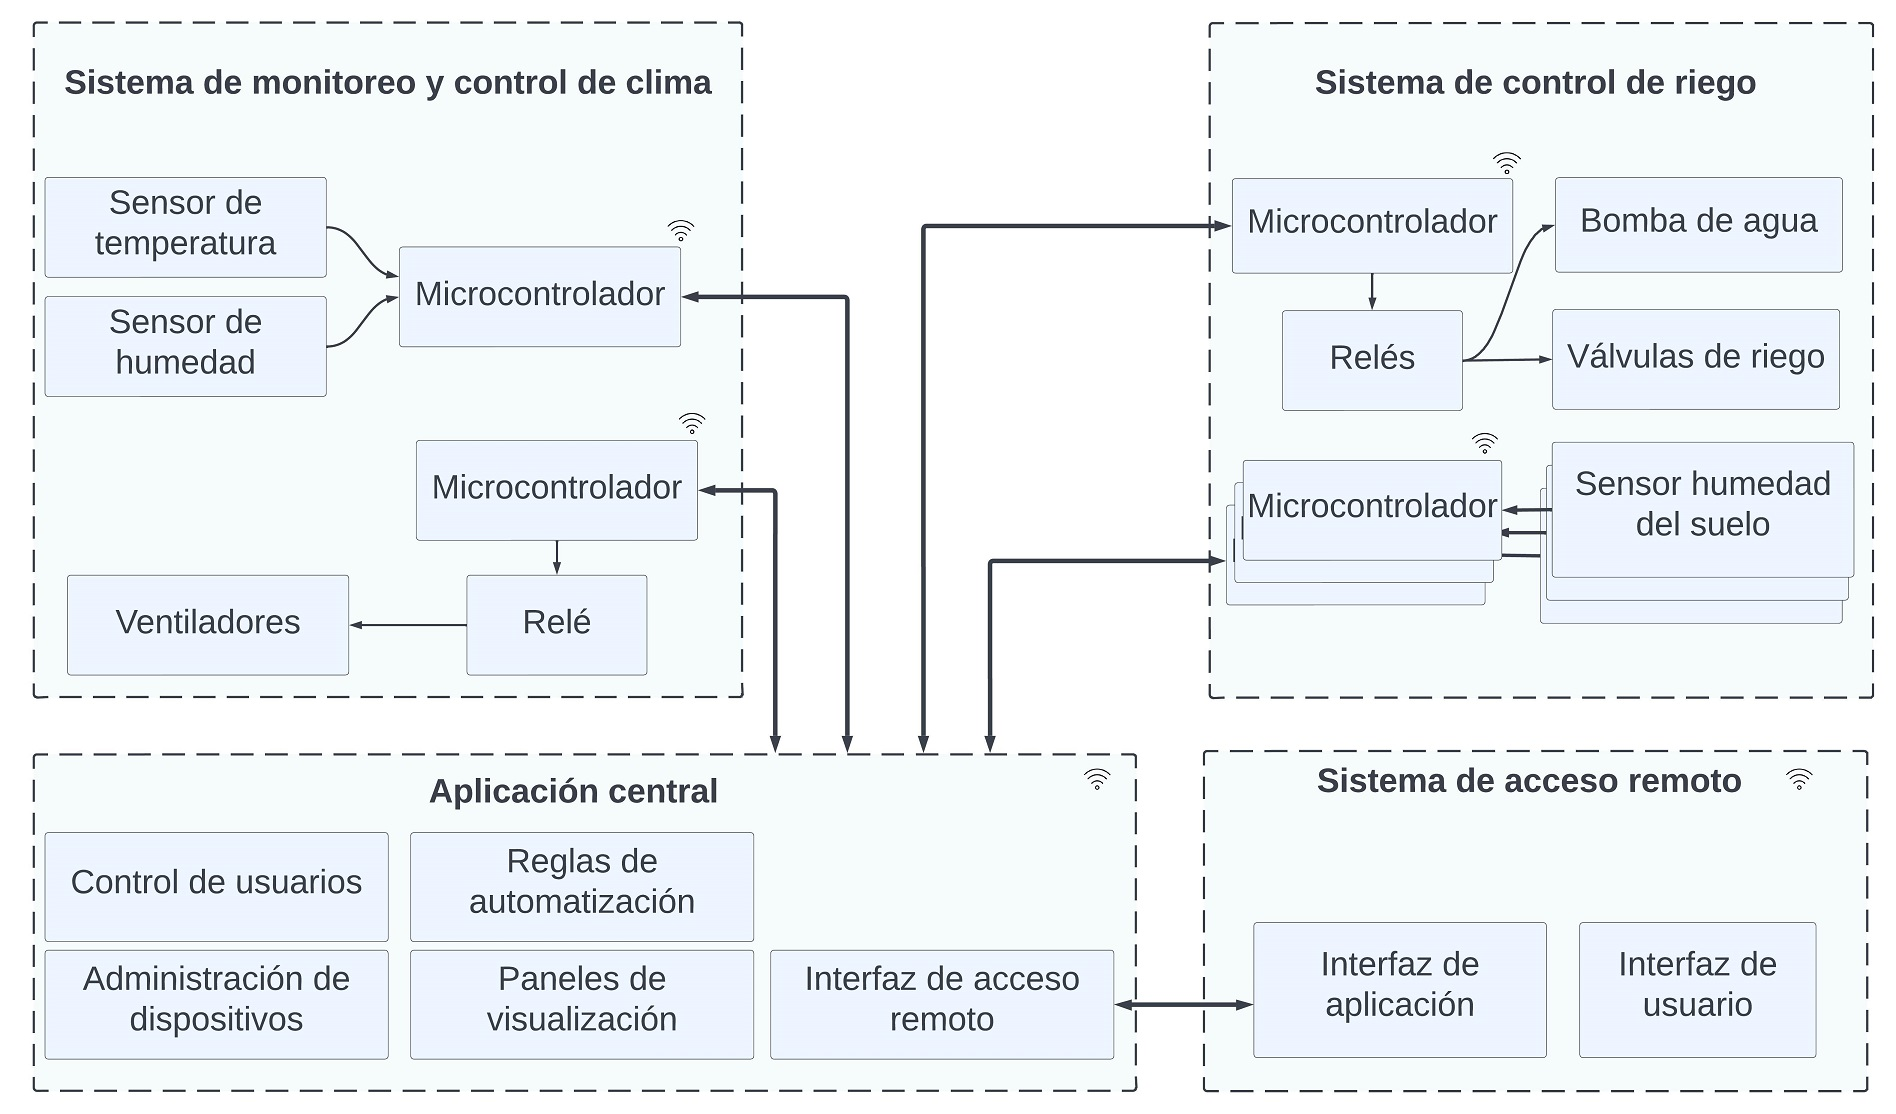
\includegraphics[width=1.0\textwidth]{./Figures/blockdiagram4.jpg}
	\caption[Arquitectura del sistema.]{Arquitectura del sistema.}
	\label{fig:blockdiagram}

\end{figure}
%
%\item Módulo de monitoreo de clima: es responsable de sensar la temperatura y humedad ambiente en el invernadero y enviar estas variables a la aplicación central para determinar las acciones a tomar en cuanto al control del clima.

%\item Sistema de control de riego: está compuesto por múltiples sensores de humedad de suelo con sus respectivos microcontroladores que se distribuyen conforme a los circuitos de riego configurados. Los sensores proceden a enviar las mediciones a la aplicación central en donde se procesan los valores y en caso de ser necesario se dispara la señal de encendido a la válvula del circuito que corresponda, y luego a la bomba de agua para así comenzar el riego. Al mismo tiempo, el usuario recibe un alerta de accionamiento de la bomba.

\item El sistema de control de riego, compuesto por dos módulos bien diferenciados:
\begin{itemize}
\item Conjunto de sensores de humedad de suelo con sus respectivos microcontroladores.
\item Unidad de control de riego constituida por un microcontrolador, relés, bomba de agua y válvulas.
\end{itemize}

Los sensores envían las mediciones a la aplicación central que se encarga de procesar los valores recibidos. En caso de ser necesario, se disparan las señales de encendido a través de la unidad de control. Primero se activa la válvula que corresponda y luego se enciende la bomba de agua para comenzar el riego. El orden de estas actividades es importante para evitar daños en la bomba o las cañerías.

\item La aplicación central que constituye el cerebro del invernadero y es la encargada de almacenar los parámetros de configuración de los diversos sensores y actuadores, procesar los mensajes recibidos, disparar acciones y alertas y visualizar el estado general.

\item El sistema de acceso remoto que permite a los usuarios obtener reportes del sistema en forma segura desde Internet.   
\end{itemize}

\subsection{Protocolos de comunicación}
\label{Protocolos de comunicación}
%\textit{Aquí se describe cómo se comunican los sistemas con la aplicación central y los protocolos usados en cada caso.}

%En la selección del software de la aplicación central se contempló la compatibilidad con múltiples protocolos de comunicación. Sin embargo limitaciones de configuración específicas, tal como el tiempo de retención de los mensajes en las colas de MQTT, forzaron el utilizar diferentes protocolos dependiendo del módulo en cuestión. Otro factor condicionante, como se detalla en la sección \ref{sec:Ciberseguridad del sistema}, fue el carecer de una CA que emita certificados que todos los componentes puedan confiar.

En esta sección se describe cómo se comunican los sistemas con la aplicación central y los protocolos usados en cada caso. En la figura \ref{fig:blockprotos} se aprecia un esquema simplificado que ilustra dichas interacciones.

Si bien tanto los módulos de hardware como el software soportan una gran variedad de protocolos,  se implementó MQTT en la mayoría de los casos conforme a los requerimientos. En algunas situaciones donde esto no fue técnicamente posible, se utilizó HTTP. Adicionalmente, para garantizar la seguridad de las comunicaciones, se incorporó un certificado autofirmado TLS en el servidor.

\begin{figure}[h]
	\centering
	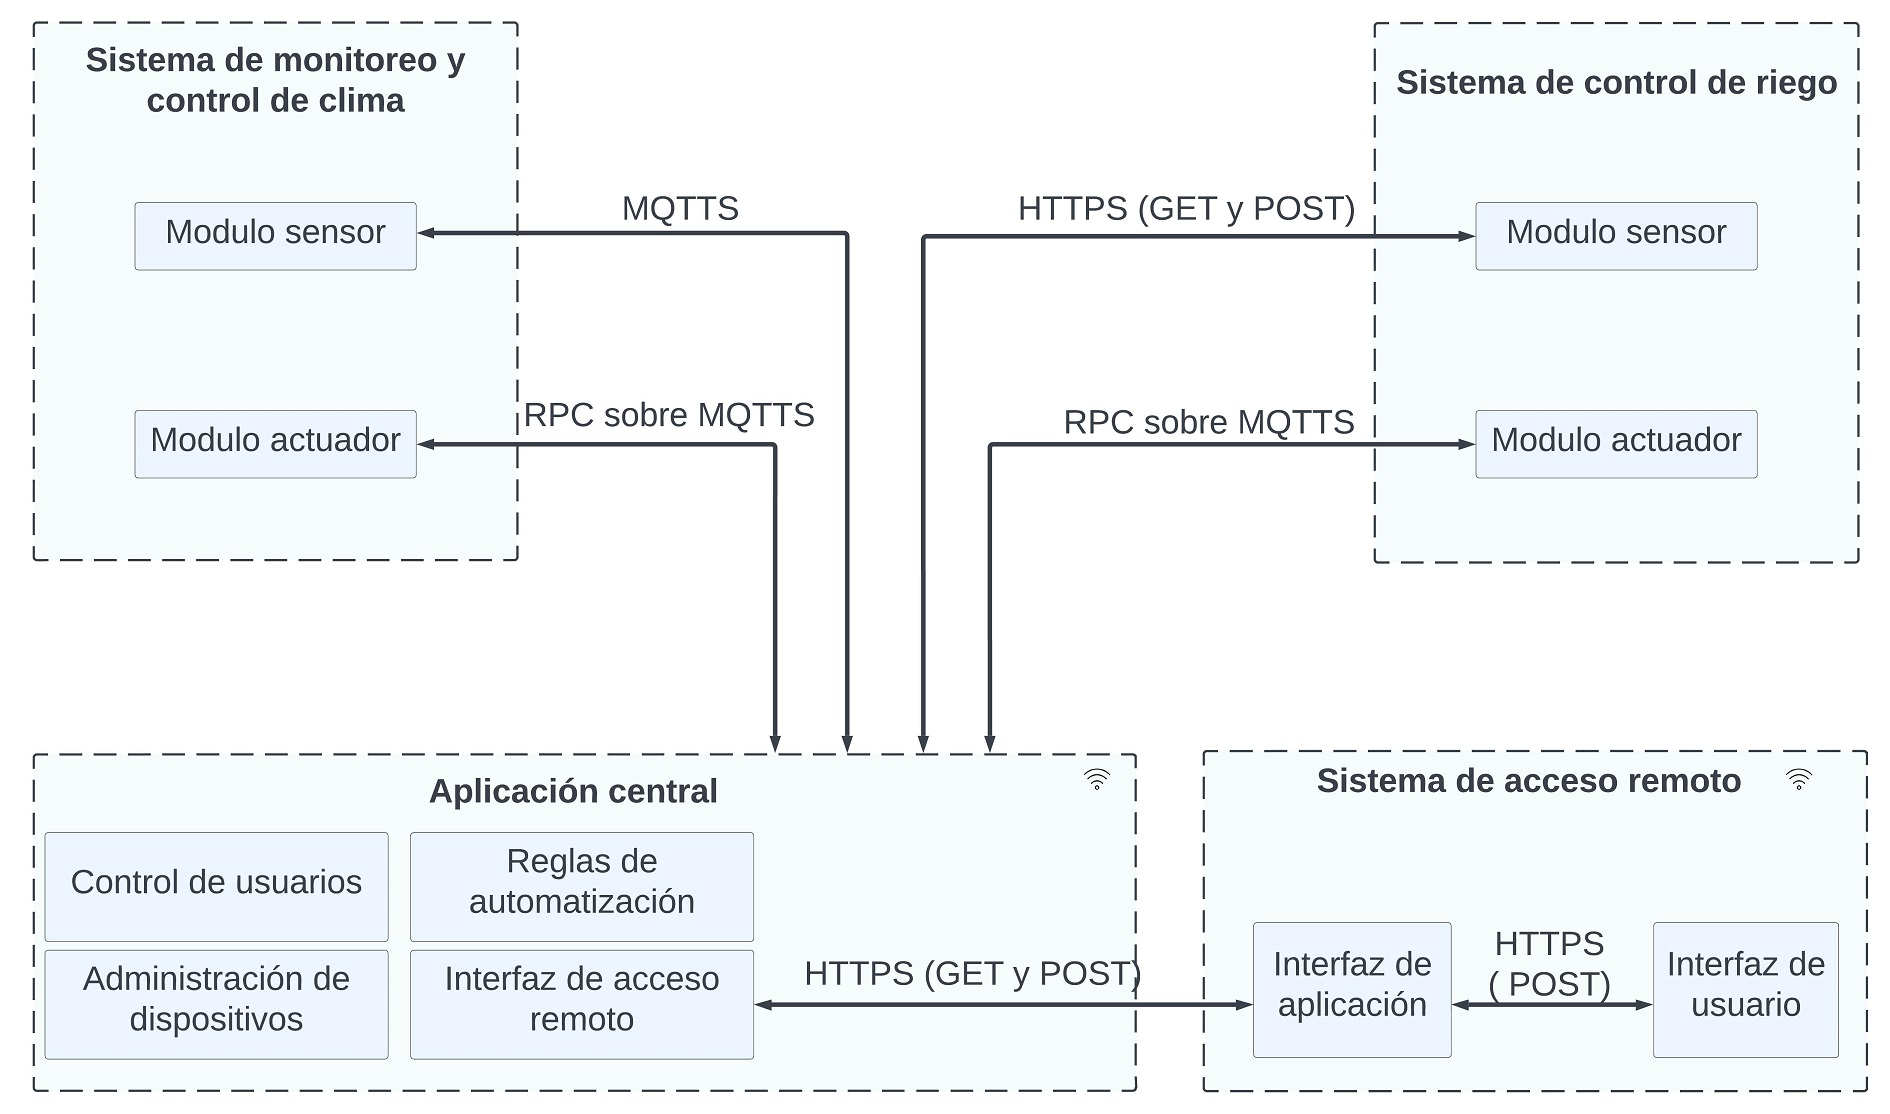
\includegraphics[width=1.0\textwidth]{./Figures/blockproto2.jpg}
	\caption[Protocolos de comunicación entre módulos.]{Protocolos de comunicación entre módulos.}
	\label{fig:blockprotos}
\end{figure}


\pagebreak
 A continuación se describen las interacciones principales entre los bloques componentes de la arquitectura:
 
 \begin{itemize}
	\item Sistema de monitoreo y control de clima: las comunicaciones desde y hasta este sistema son con la aplicación central.
	El módulo sensor envía las mediciones realizadas por medio de MQTT.
	En el caso que las variables del clima requieran una acción, la aplicación central comanda el encendido de los ventiladores por medio de un mensaje enviado por RPC \citep{rfc1057} sobre MQTT.
	
	\item Sistema de control de riego: las comunicaciones desde y hasta este sistema son con la aplicación central.
	El módulo sensor realiza dos conexiones, una para el envío de las mediciones y otra para recibir variables de configuración tales como el período de \textit{deep sleep}. Debido a limitaciones en la configuración de la persistencia de los mensajes en las colas de MQTT, se optó por utilizar llamadas HTTP (GET y POST) para realizar estas comunicaciones.
	Al igual que en el control de clima, la aplicación central inicia el riego por medio de mensajes RCP sobre MQTT hacia el controlador de la bomba y de las válvulas.
	
	\item Sistema de acceso remoto: la interfaz se comunica con la aplicación por medio de pedidos HTTP GET y POST para consultar el reporte de estado de los diferentes componentes. A continuación este se envia hacia la interfaz de usuario por medio de una solicitud HTTP POST.
 
 
 
 
 \end{itemize}






\section{Detalle de los módulos de hardware}
\label{sec:Módulos de hardware}
En esta sección se describen en detalle los esquemas de conexión de los distintos módulos y las consideraciones de diseño y construcción empleadas. 

\subsection{Módulos sensores de humedad del suelo}
\label{Módulos sensores de humedad del suelo}


En el proyecto se desarrollaron dos configuraciones distintas de módulos para medir humedad del suelo en macetas de distinto tipo y tamaño. Ambas opciones utilizan el microcontrolador ESP8266 pero incorporan un distinto número de sensores. En la figura \ref{fig:soilschem1} se muestra el esquema de conexión para la versión simple (con un único sensor) y en la figura \ref{fig:soilschem2} se ilustra la configuración doble.

Si bien en el prototipo los sensores se conectaron a una fuente de alimentación, la configuración y conexión del sistema está optimizada para el uso de baterías. Esto responde a que estos sensores estarán desplegados en múltiples ubicaciones dentro del invernadero, donde no siempre es posible alimentarlos con una fuente de energía. 

El ahorro de energía se logra al utilizar ciclos de apagado en los períodos donde no se realizan lecturas. A este mecanismo se lo conoce como \textit{deep sleep} y se implementó por medio de un puente entre los pines A0 (GPIO0) y RST del chip ESP8266. Esta conexión le permite reactivarse luego de un período de hibernación por medio de su reloj interno. En base a esta funcionalidad se logra una reducción del consumo de energía a valores muy pequeños que rondan los 0,3 mA durante el período de inactividad.




\begin{figure}[!h]
     \centering
     \begin{subfigure}[b]{0.45\textwidth}
		\centering
		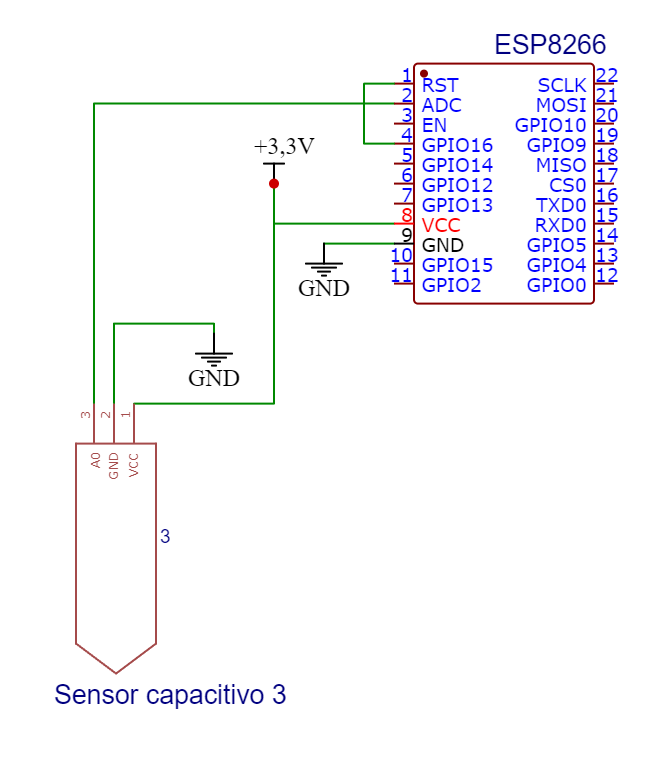
\includegraphics[width=0.9\textwidth]{./Figures/soil_schem_simple.png}
		\caption[Esquema de conexión de módulo de sensor simple]{Esquema de conexión de módulo de sensor simple.}
		\label{fig:soilschem1}
     \end{subfigure}
     \hfill
     \begin{subfigure}[b]{0.45\textwidth}
	\centering
		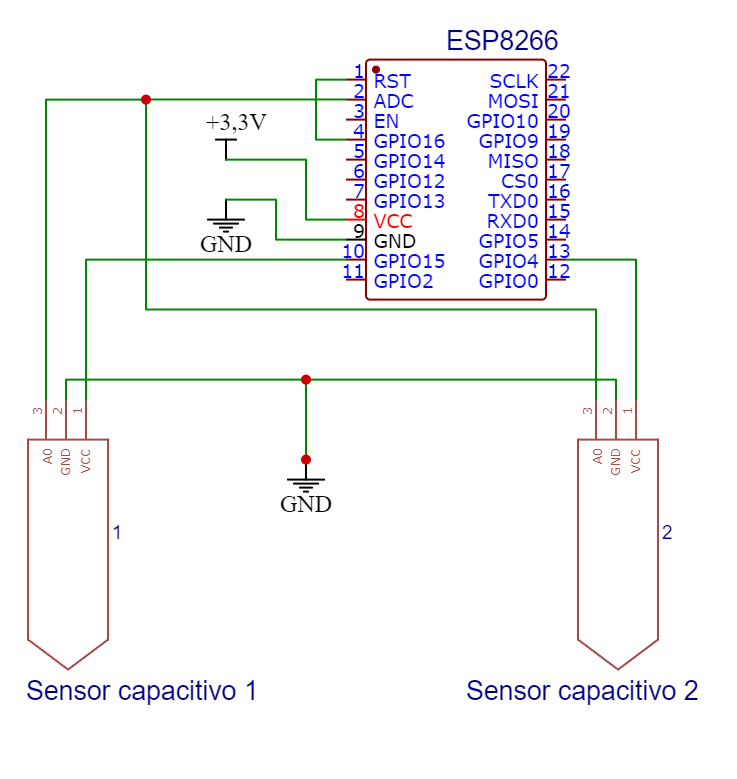
\includegraphics[width=1\textwidth]{./Figures/soil_schem_doble.png}
		\caption[Esquema de conexión de módulo de sensor doble]{Esquema de conexión de módulo de sensor doble.}
		\label{fig:soilschem2}
     \end{subfigure}
     \hfill
        \caption[Conexión del sensor de humedad del suelo]{Conexión del sensor de humedad del suelo.}	\label{fig:soilschem}
\end{figure}
%\begin{figure}[!h]
%	\centering
%	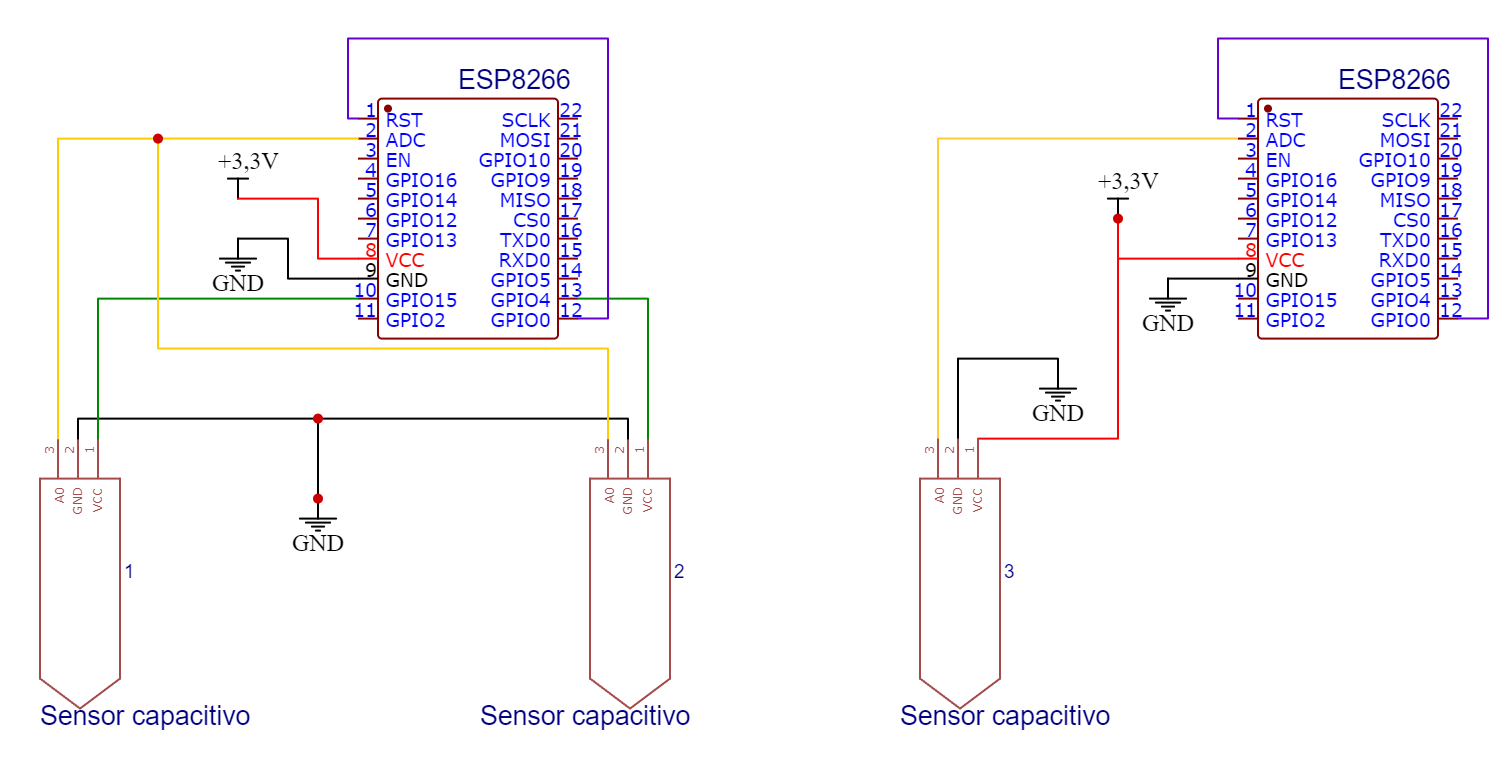
\includegraphics[width=1\textwidth]{./Figures/soil_schematic2.png}
%	\caption[Conexión del sensor de humedad del suelo]{Conexión del sensor de humedad del suelo.}
%	\label{fig:soilschem}
%\end{figure}

Dado que estos dispositivos están sujetos a riesgos de salpicaduras o contacto con agua, se procedió a cubrir la electrónica expuesta de los sensores mediante el uso de tubos adhesivos termocontraibles, los cuales al aplicarles calor generan una sello a prueba de agua. Para la protección del chip ESP8266, se utilizó una caja de polipropileno transparente sellada. En las figuras \ref{fig:soil3} y \ref{fig:soil4} se muestran los componentes y sus protecciones. 

\begin{figure}[!h]
     \centering
     \begin{subfigure}[b]{0.45\textwidth}
		\centering
		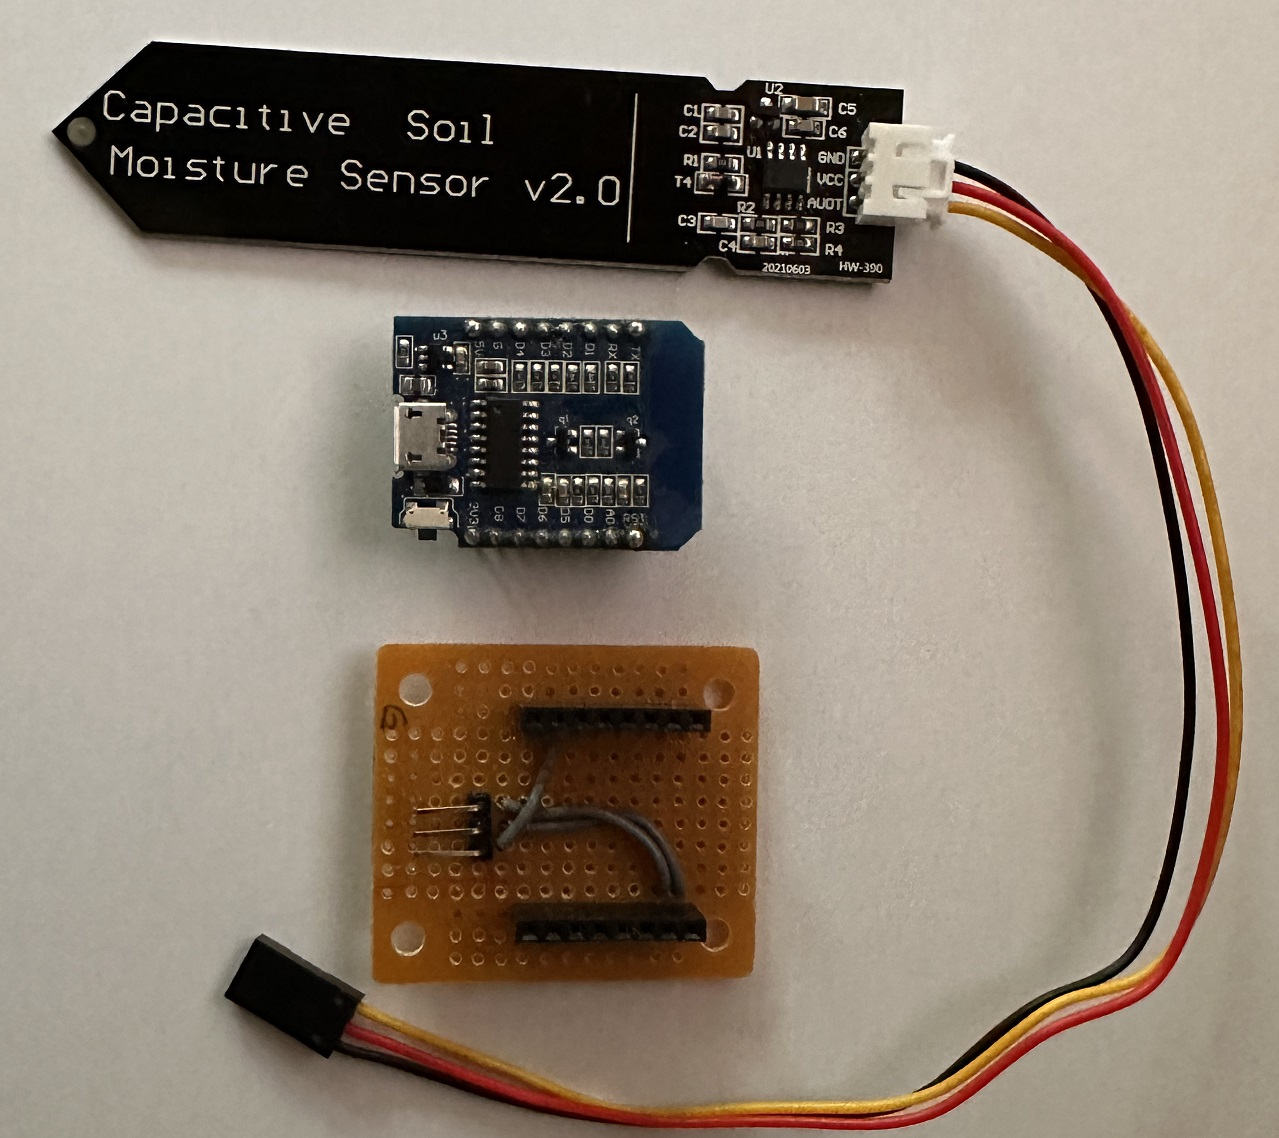
\includegraphics[width=0.60\textwidth]{./Figures/soil1.jpeg}
		\caption[Módulo con un sensor de humedad del suelo]{Módulo con un sensor de humedad del suelo.}
		\label{fig:soil1}
     \end{subfigure}
     \hfill
     \begin{subfigure}[b]{0.45\textwidth}
	\centering
		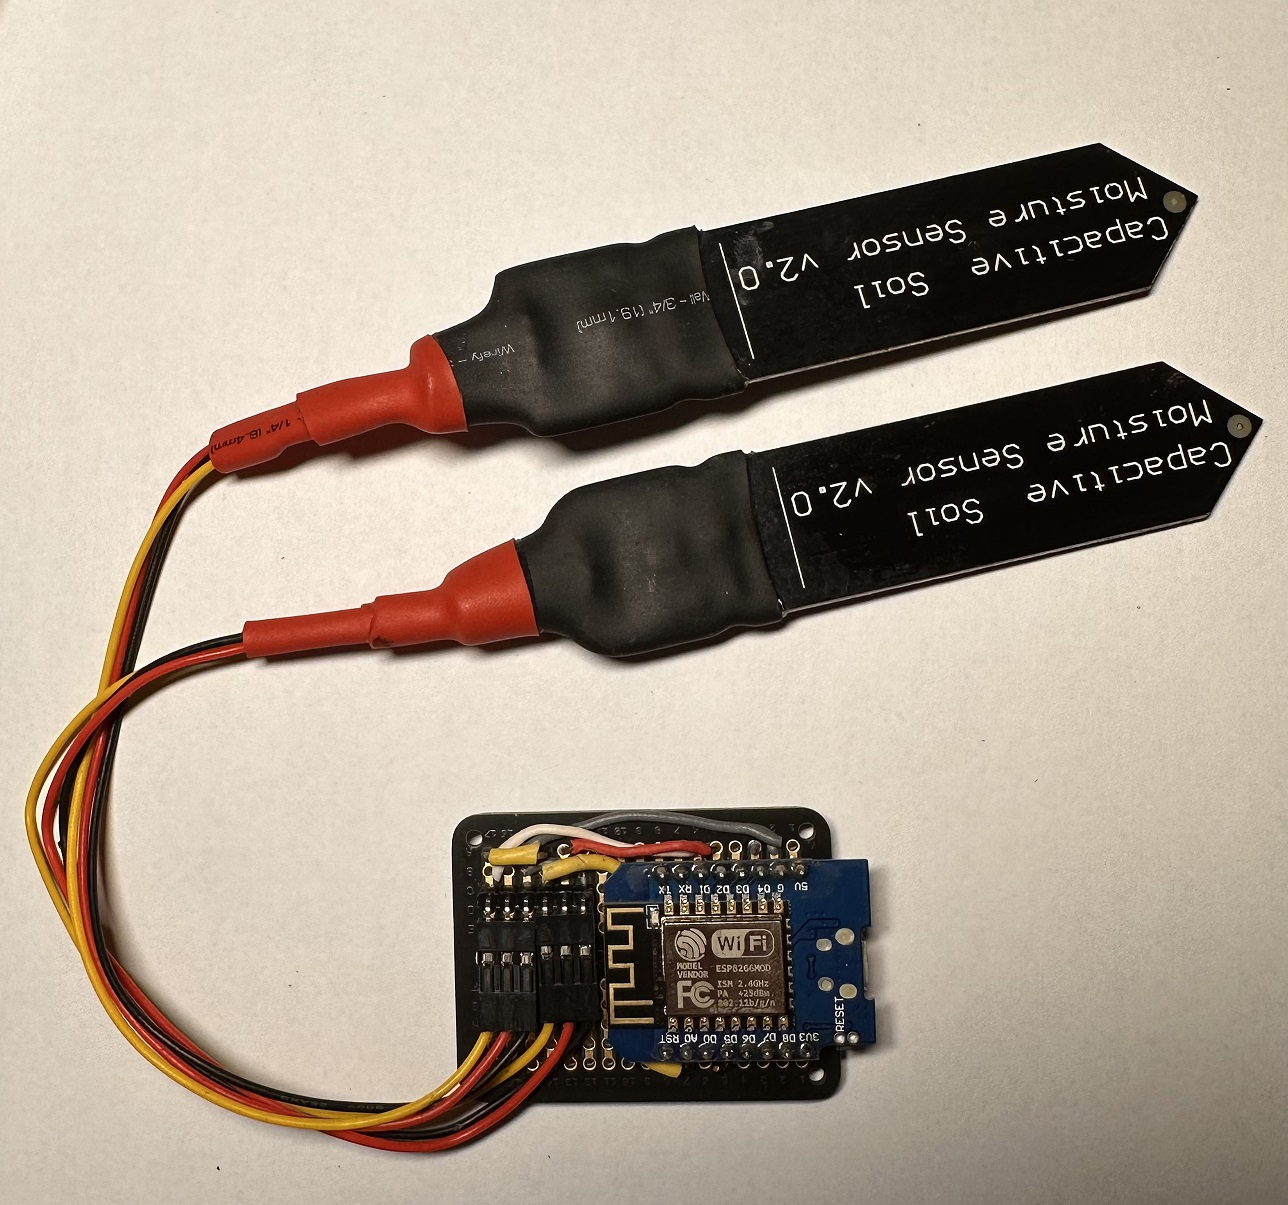
\includegraphics[width=0.60\textwidth]{./Figures/soil2.jpeg}
		\caption[Módulo con dos sensores de humedad del suelo]{Módulo con dos sensores de humedad del suelo.}
		\label{fig:soil2}
     \end{subfigure}
      \begin{subfigure}[b]{0.45\textwidth}
	\centering
		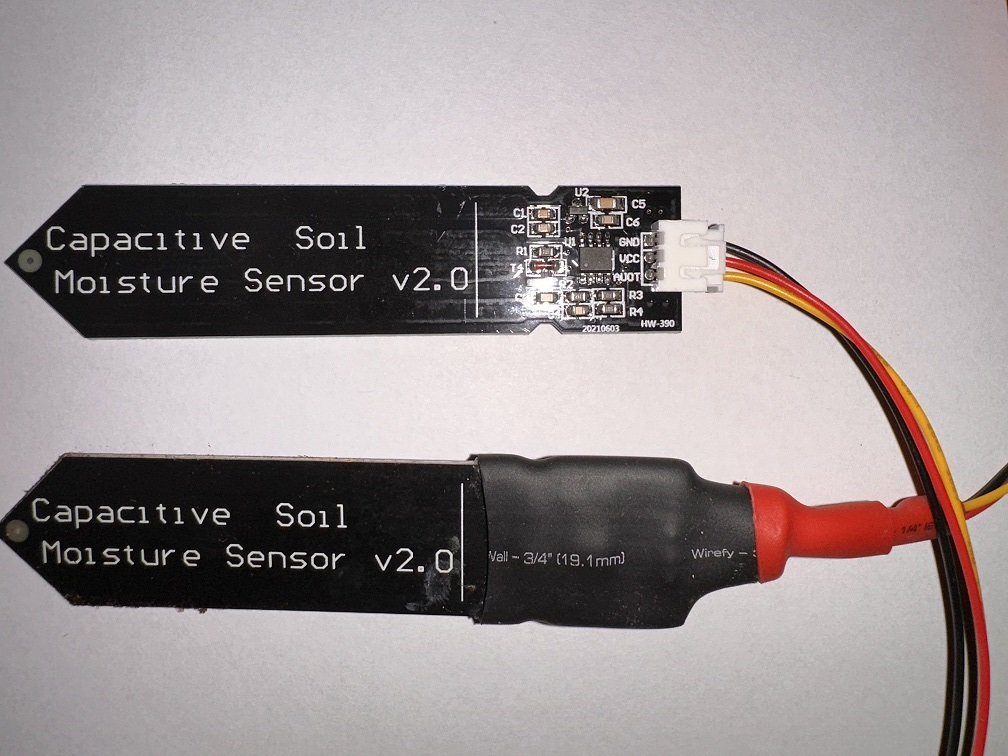
\includegraphics[width=0.60\textwidth]{./Figures/soil_compare.jpg}
		\caption[Detalle de protección de circuitos en los sensores]{Detalle de protección de circuitos en los sensores.}
		\label{fig:soil3}
     \end{subfigure}	
			\begin{subfigure}[b]{0.45\textwidth}
	\centering
		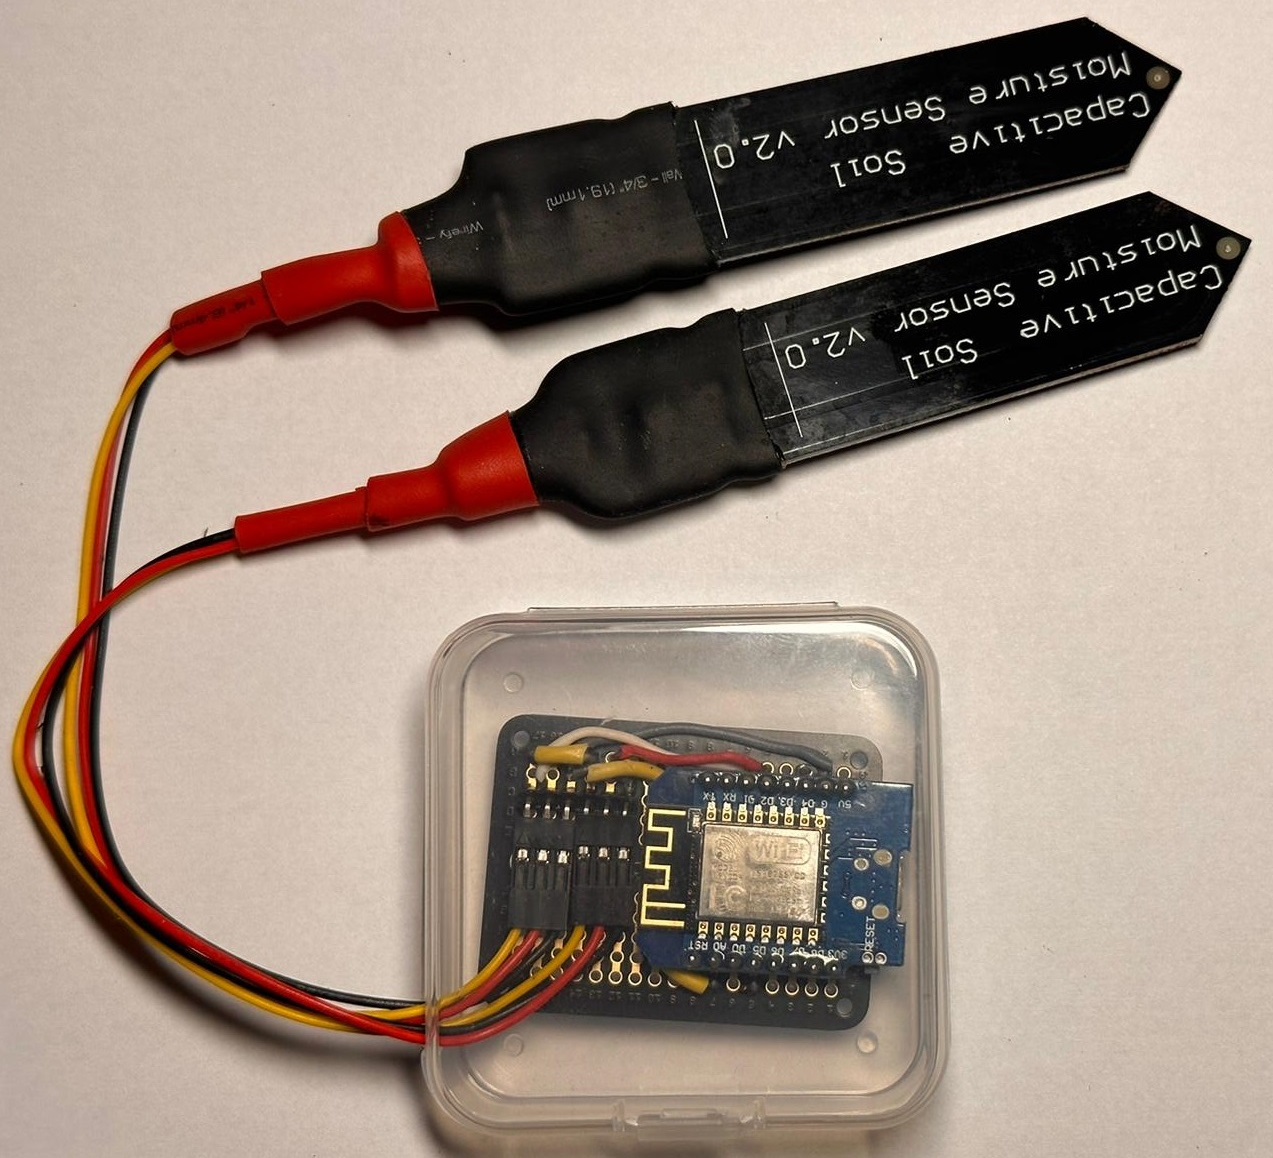
\includegraphics[width=0.60\textwidth]{./Figures/soil3.jpg}
		\caption[Módulo en su caja protectora]{Módulo en su caja protectora.}
		\label{fig:soil4}
     \end{subfigure}
     \hfill
        \caption[Módulos de sensores de humendad de suelo  empleados en el proyecto]{Módulo de sensores de humendad de suelo  empleados en el proyecto.}
        \label{fig:soilsenors}
\end{figure}


\pagebreak

\subsection{Módulo controlador del riego}
\label{Módulo controlador del riego}

Este es el módulo de mayor complejidad del invernadero, se compone de un microcontrolador ESP32, una placa de interfaz de relé de cuatro canales, un regulador DC-DC \textit{step down} de voltaje LM2596 y una pantalla LCD/OLED SSH1106. El esquema de conexiones entre estos componentes se detalla en la fig \ref{fig:riegochem}.

El sistema está conectado a fuente de 12 VDC, que alimenta adicionalmente al conjunto de bomba y válvulas de riego. Al pasar por el regulador LM2596, la tensión es reducida a 5 VDC para alimentar al ESP32, la pantalla y el circuito de control del relé.

\begin{figure}[!h]
	\centering
	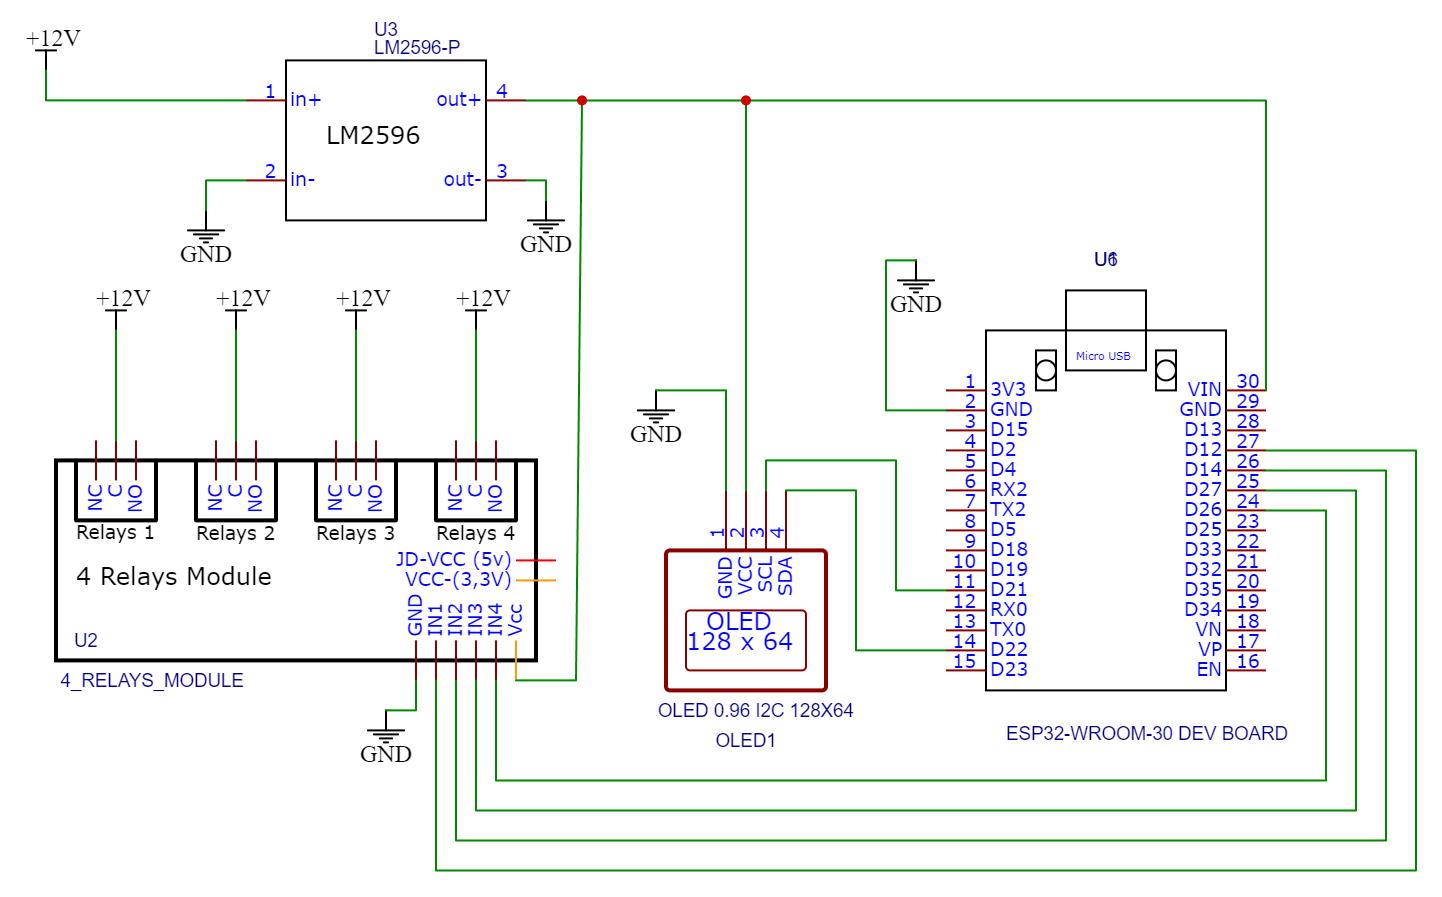
\includegraphics[width=0.9\textwidth]{./Figures/pump_schem.png}
	\caption[Conexión del modulo de control de riego]{Conexión del modulo de control de riego.}
	\label{fig:riegochem}
\end{figure}

\begin{figure}[!h]
	\centering
	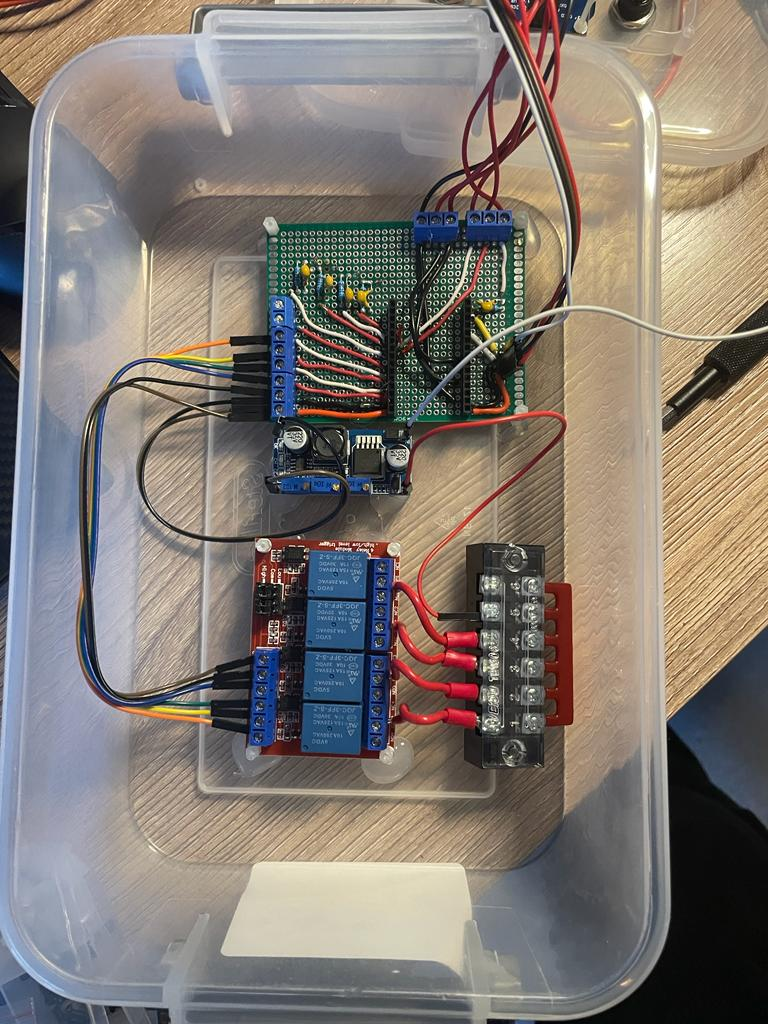
\includegraphics[width=0.5\textwidth]{./Figures/riego1.jpg}
	\caption[Modulo completo en su caja protectora]{Modulo completo en su caja protectora.}
	\label{fig:riego_control}
\end{figure}
 
\pagebreak

\subsection{Módulo sensor de temperatura y humedad}
\label{Módulo sensor de temperatura y humedad}

Compuesto por un microcontrolador ESP8266, un sensor DHT22, al que se le integra una pantalla LCD/OLED SSH1106 para visualizar los valores de temperatura y humedad  \textit{in situ} en tiempo real. 
Para la construcción se utilizó una caja de polipropileno transparente a la que se adaptó para la entrada de alimentación y la exposición del DHT22. 


\begin{figure}[!h]
	\centering
	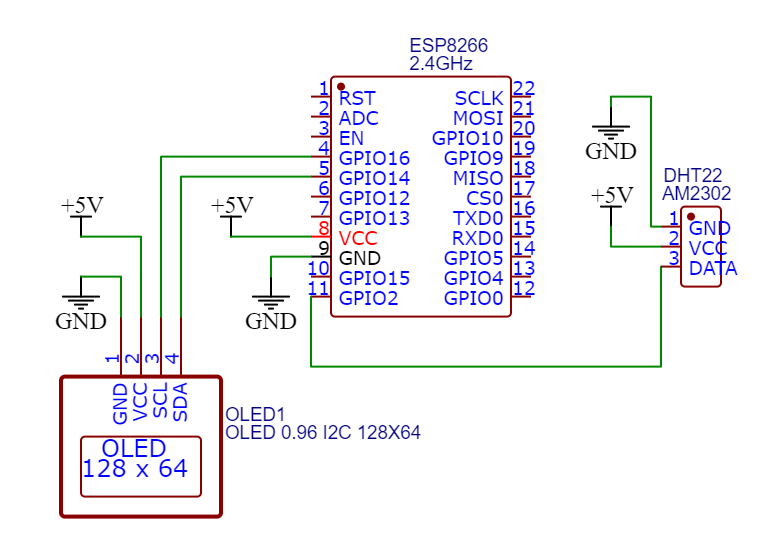
\includegraphics[width=0.7\textwidth]{./Figures/temp_sensor.png}
	\caption[Conexión del sensor de temperatura y humedad]{Conexión del sensor de temperatura y humedad
	.}
	\label{fig:tempschem}
\end{figure}


\begin{figure}[!h]
	\centering
	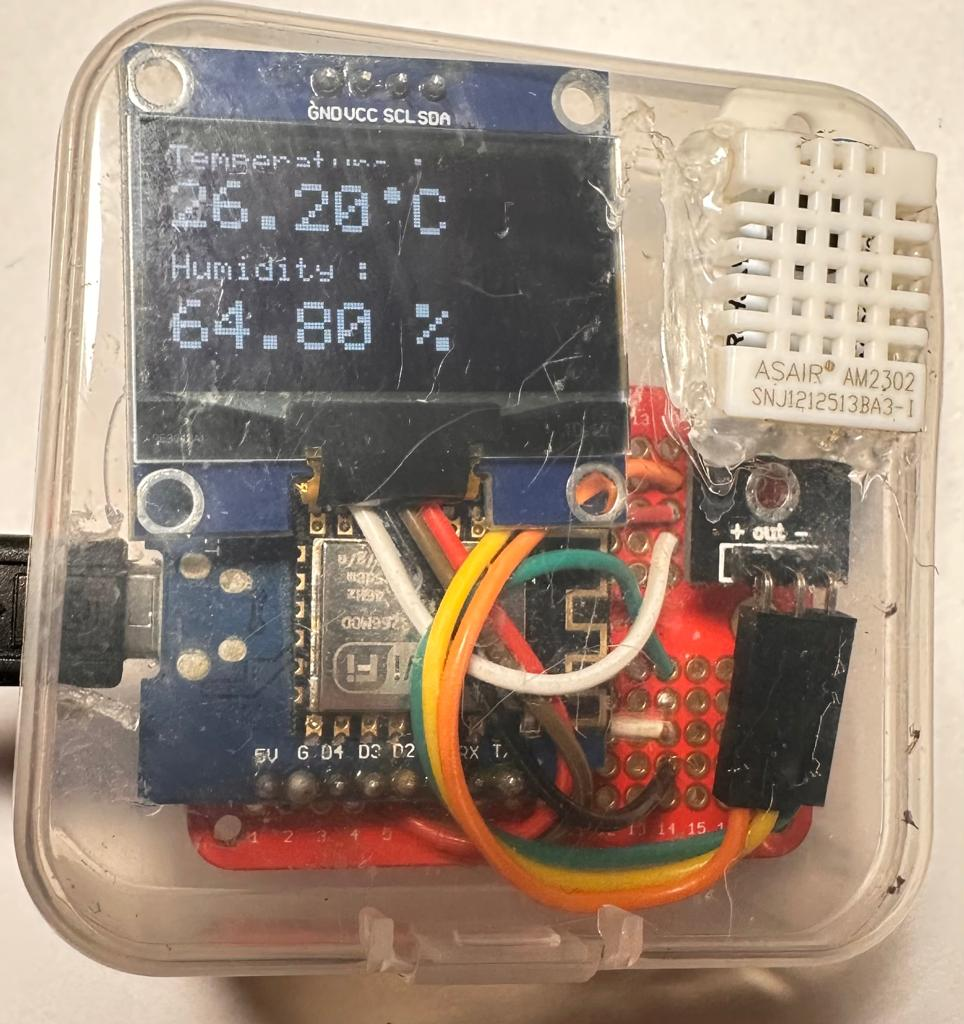
\includegraphics[width=0.5\textwidth]{./Figures/sensor_temp.jpg}
	\caption[Modulo completo en su caja protectora]{Modulo completo en su caja protectora.}
	\label{fig:temp_sensor}
\end{figure}

\pagebreak
\subsection{Módulos controladores de clima}
\label{Módulos controladores de clima}

El módulo responsable de accionar los ventiladores en el invernadero. Para la construcción se utilizó un ESP8266 conectado a un relé de una vía. Dado que la salida del microcontrolador es de 3,3 V y la activación del relé es de 5V, se evaluó incorporar un convertidor de tensión DC-DC \textit{step up}, pero luego de las pruebas realizadas se comprobó que no era necesario. 

\begin{figure}[!h]
	\centering
	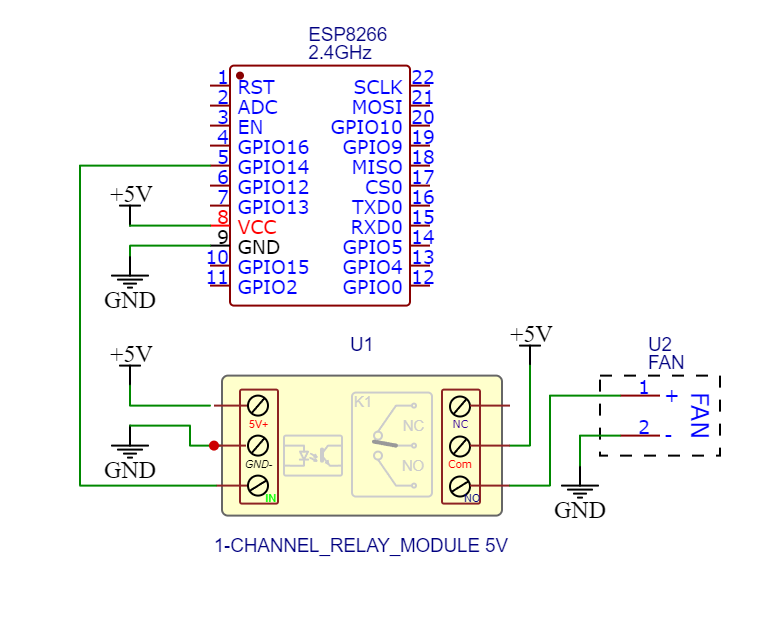
\includegraphics[width=0.7\textwidth]{./Figures/vent_schem.png}
	\caption[Conexión del modulo de control de clima]{Conexión del modulo de control de clima.}
	\label{fig:ventschem}
\end{figure}


\begin{figure}[!htpb]
     \centering
     \begin{subfigure}[b]{0.45\textwidth}
		\centering
		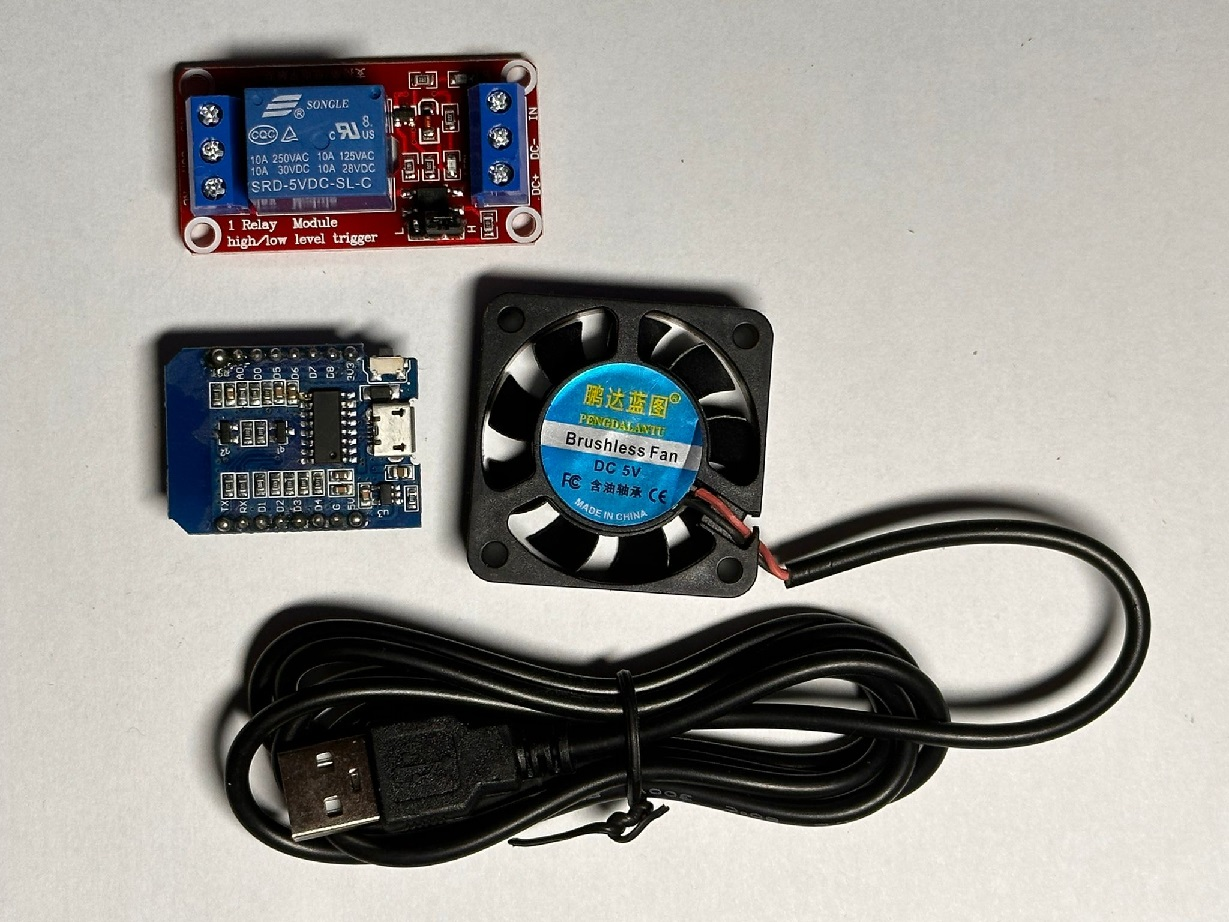
\includegraphics[width=0.80\textwidth]{./Figures/vent_control.jpg}
		\caption{Detalle de los componentes.}
		\label{fig:vent1}
     \end{subfigure}
     \hfill
     \begin{subfigure}[b]{0.45\textwidth}
	\centering
		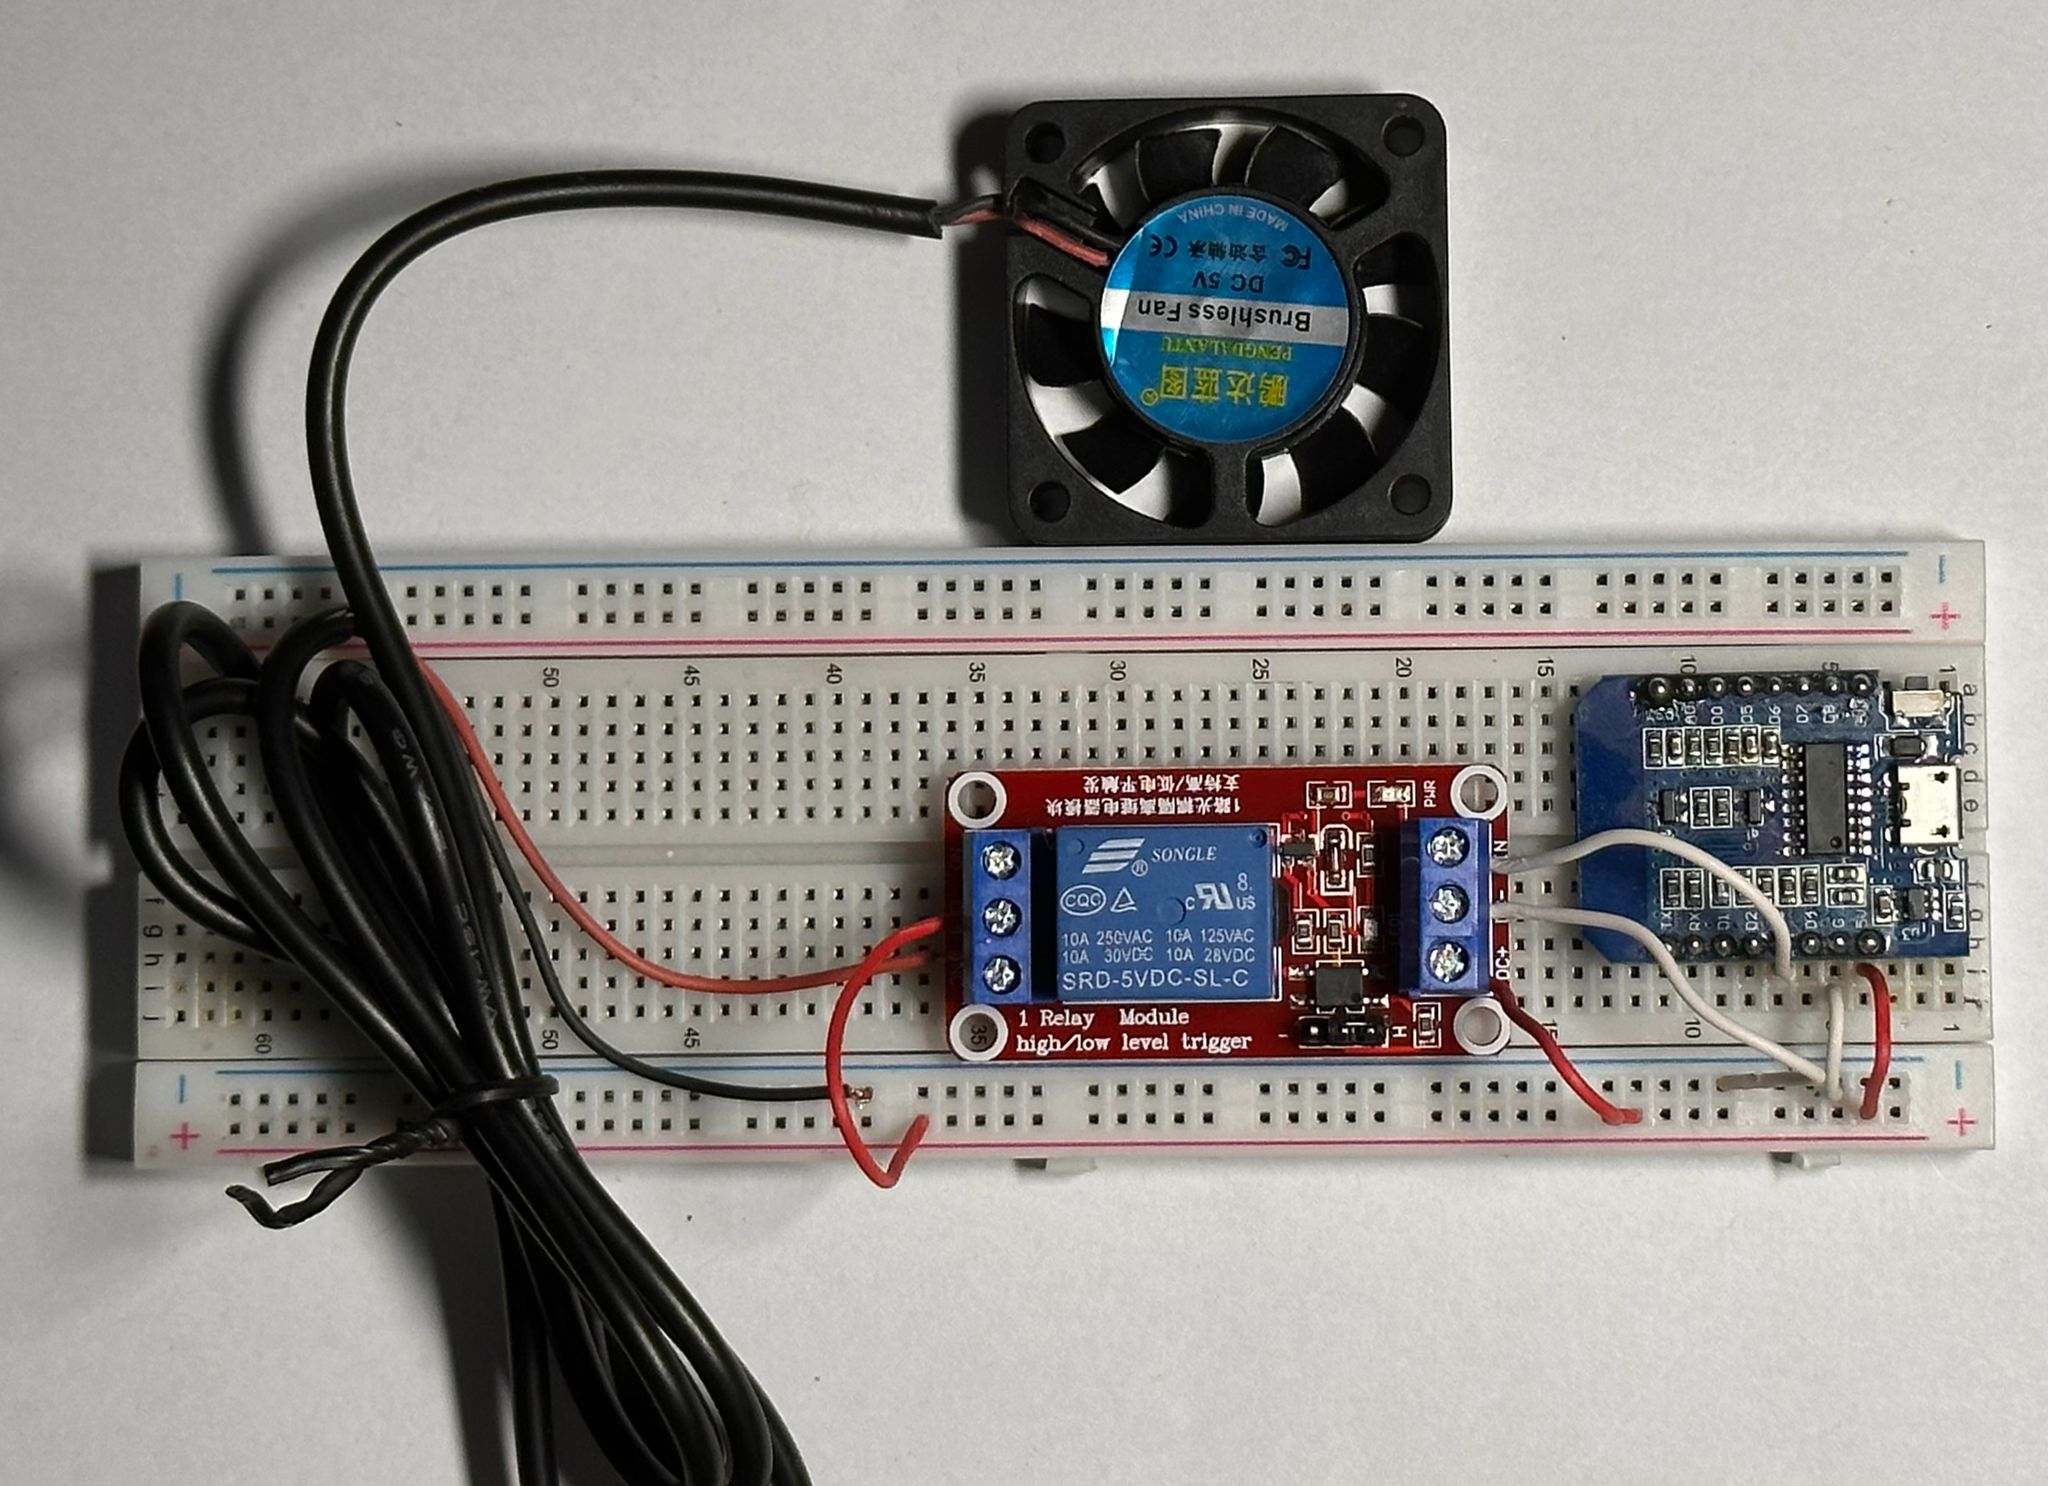
\includegraphics[width=0.80\textwidth]{./Figures/vent_proto.jpg}
		\caption{Configuración del módulo.}
		\label{fig:vent2}
     \end{subfigure}	
	\begin{subfigure}[b]{0.45\textwidth}
		\centering
		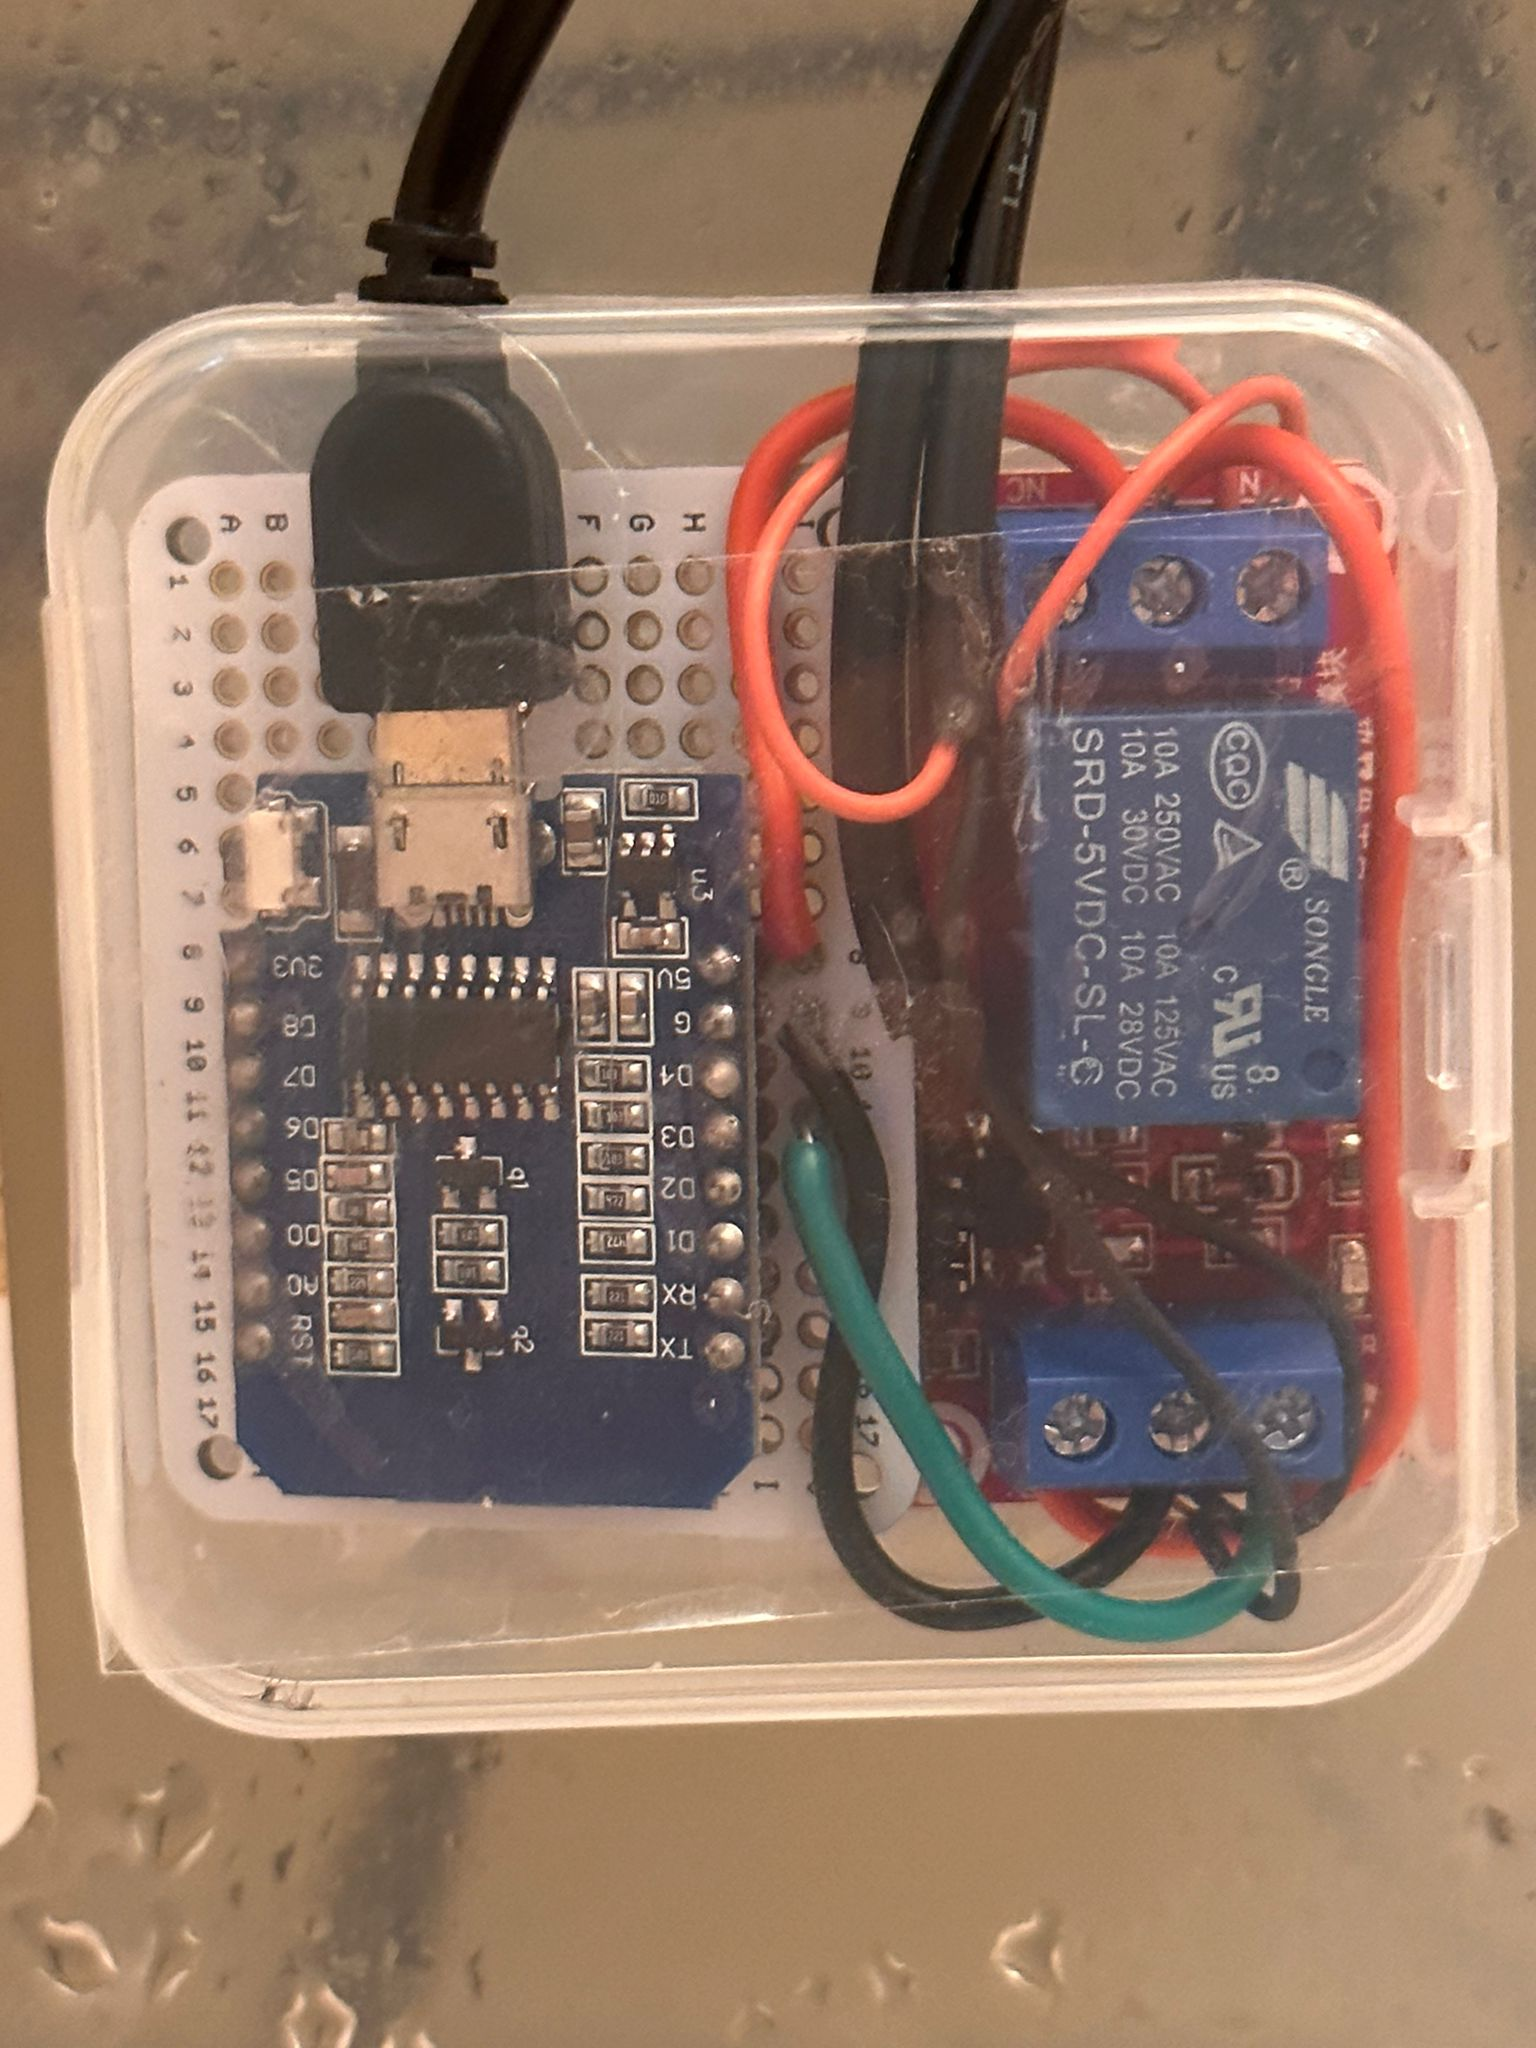
\includegraphics[width=0.60\textwidth]{./Figures/vent_assembled.jpg}
		\caption{Módulo finalizado en su caja protectora.}
		\label{fig:vent3}
     \end{subfigure}
     \hfill
        \caption[Módulo de control del clima]{Módulo de control del clima.}
        \label{fig:soilsenors}
\end{figure}


\pagebreak

\section{Detalle del firmware desarrollado}
\label{sec:Desarrollo del firmware}


%\subsection{Programación del microcontrolador de medición de clima}
%\label{Programación del microcontrolador de medición de clima}


\section{Selección y configuración del software}
\label{sec:Selección y configuración del software}

\section{Ciberseguridad del sistema}
\label{sec:Ciberseguridad del sistema}
